
\begin{frame}{Overview}
  Our UI2I transformation consists of:
  \begin{enumerate}
    \item A deep UI2I estimator.
    \item A physical estimator calibrated to perform thermal UI2I.
    \item Fusion of deep and physical estimators (PETIT-GAN).
  \end{enumerate}
\end{frame}

\subsection{Deep Estimator}
\begin{frame}{Models}
  \begin{itemize}
    \item Generative Adversarial Networks(GANs): generator \vs discriminator/critic. \hyperlink{apndx:gan}{\beamerbutton{GAN architecture}}
    \item Two SOTA UI2I GANs were examined:
    \begin{enumerate}
      \item CycleGAN \cite{CycleGAN2017} (cycle consistency). \hyperlink{apndx:cycle_gan}{\beamerbutton{CycleGAN architecture}}
      \item Contrastive Unpaired Translation (CUT) \cite{park2020cut} (contrastive learning). \hyperlink{apndx:cat}{\beamerbutton{CUT architecture}}
    \end{enumerate}
  \end{itemize}
  \begin{figure}
    \centering
    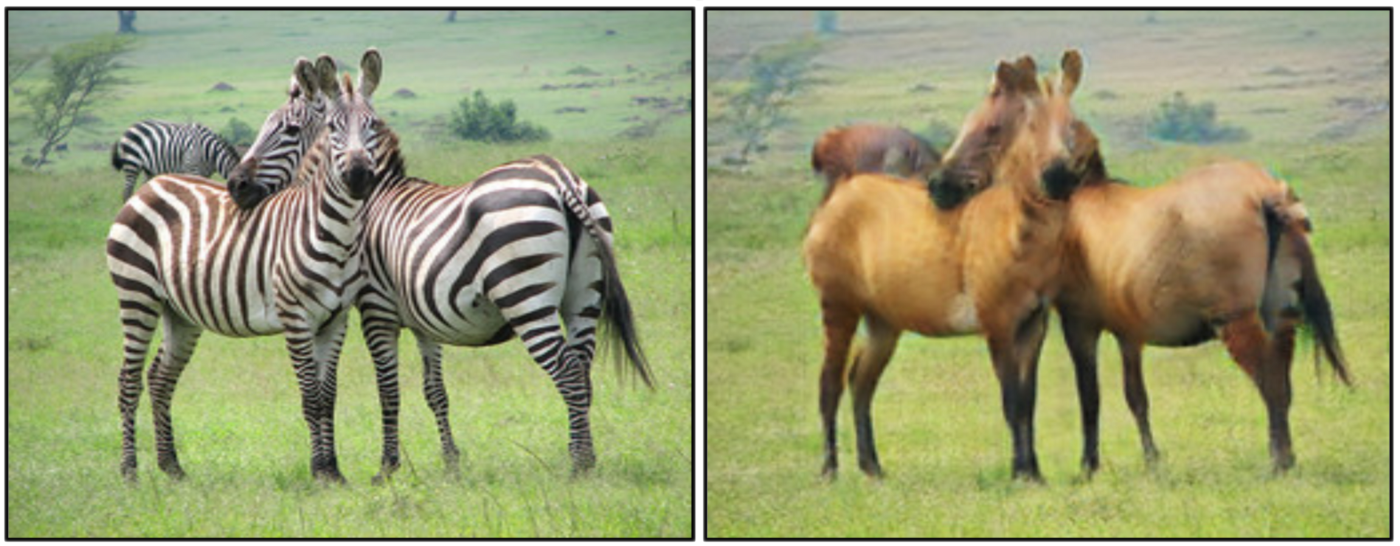
\includegraphics[width=0.5\linewidth]{../figs/related_work/horses_to_zebras.png}
  \end{figure}  
\end{frame}

\begin{frame}{Generator architecture}
  \begin{itemize}
    \item Both models share the same generator implementation.
    \begin{figure}
      \centering
      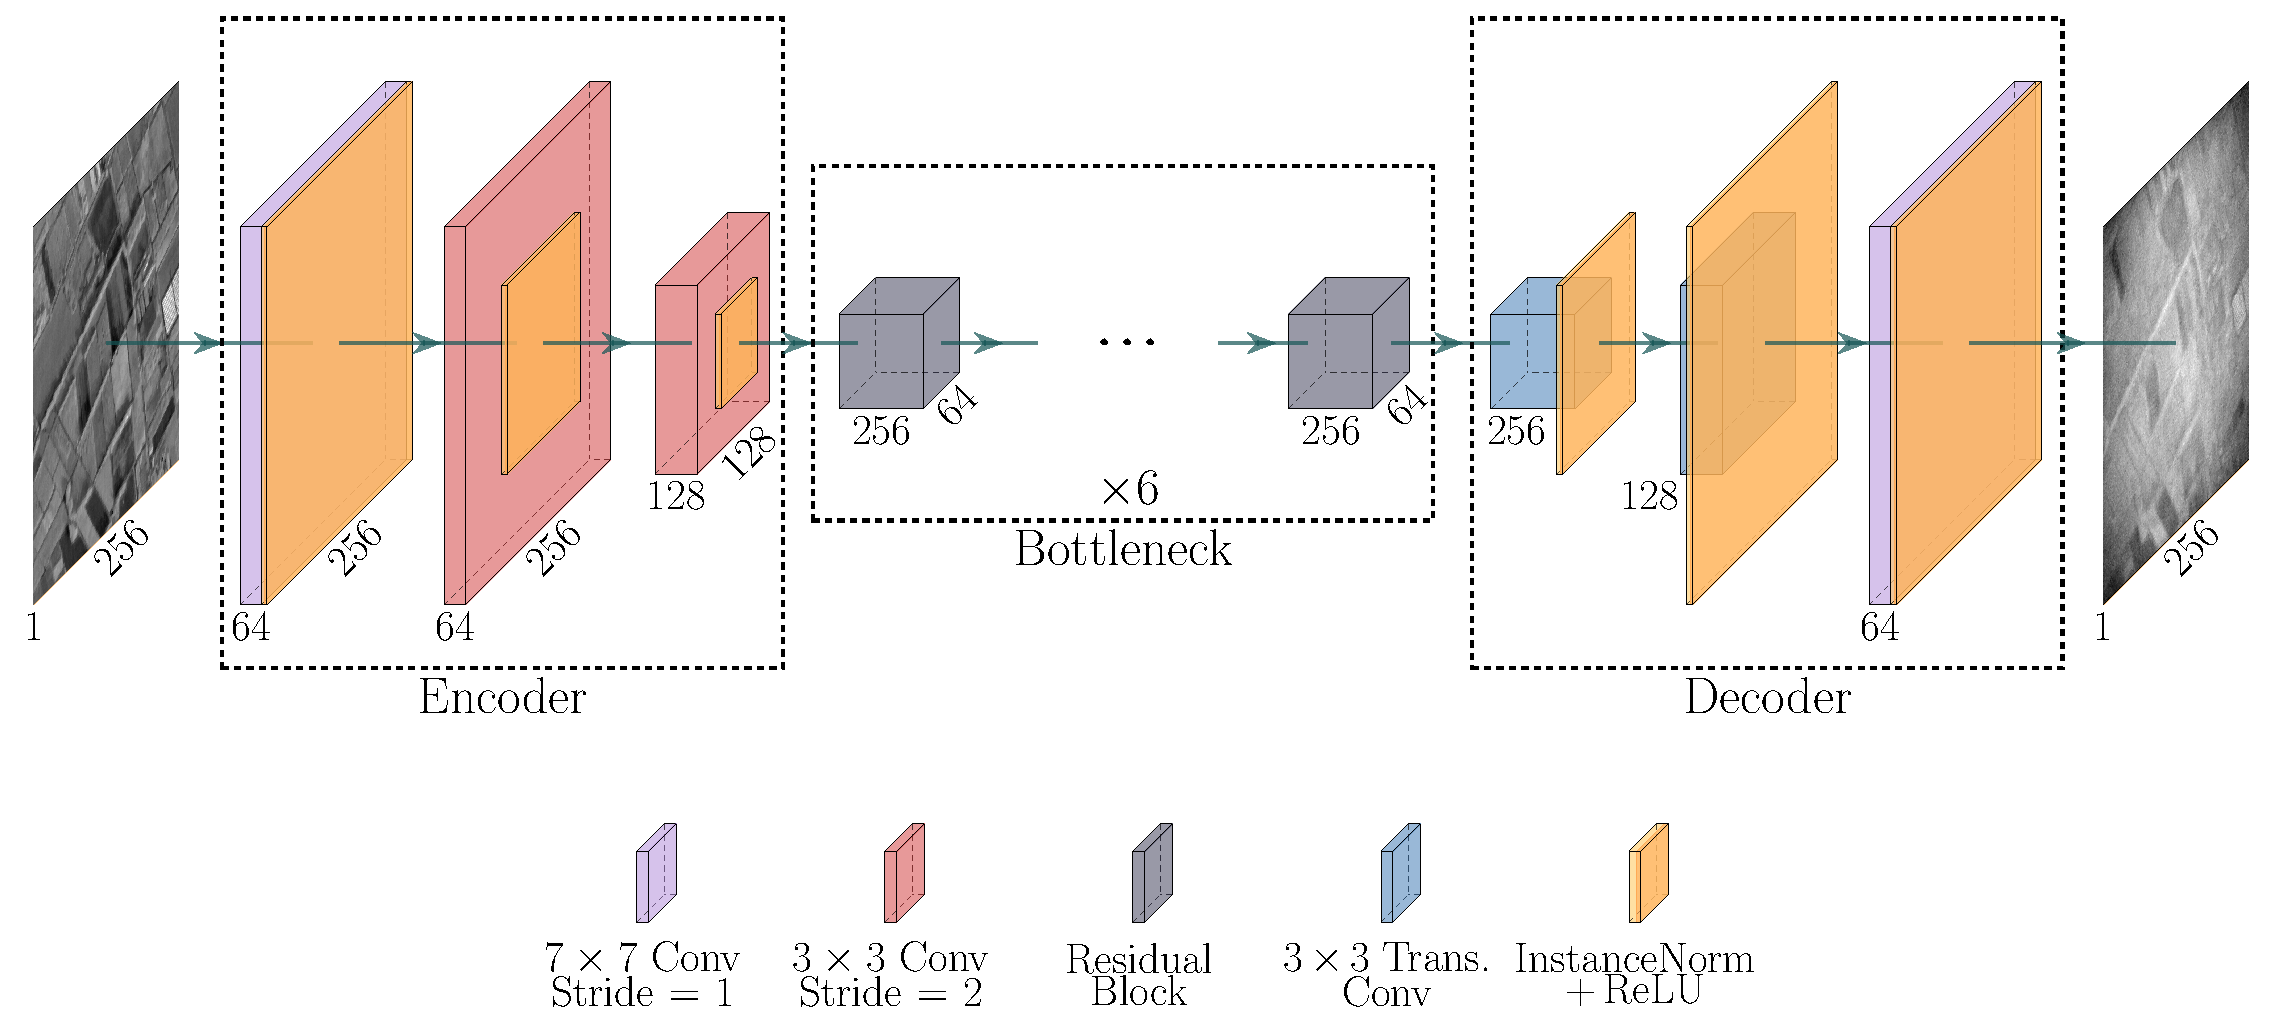
\includegraphics[width=\linewidth]{../figs/network/src/cut.pdf}
    \end{figure}  
  \end{itemize}
\end{frame}

\subsection{Physical Estimator}

\begin{frame}{Bakcground}
  \emph{Blackbody Radiation}: electromagnetic emission of an ideal opaque object due to its temperature.
  \setlength\abovedisplayskip{0pt}
  \begin{exampleblock}{Stephan-Boltzmann}
    \begin{equation*} \label{eq:stephan-boltzmann-ideal}
      P(T) = \int_0^\infty \frac{2\pi hc^2}{\lambda^5}\frac{1}{e^{\frac{hc}{\lambda kT}} - 1} d\lambda = \frac{\sigma}{\pi} T^4 \; \; \left[W sr^{-1} m^{-2}\right]
    \end{equation*}
  \end{exampleblock}  
  \begin{figure}
    \centering
    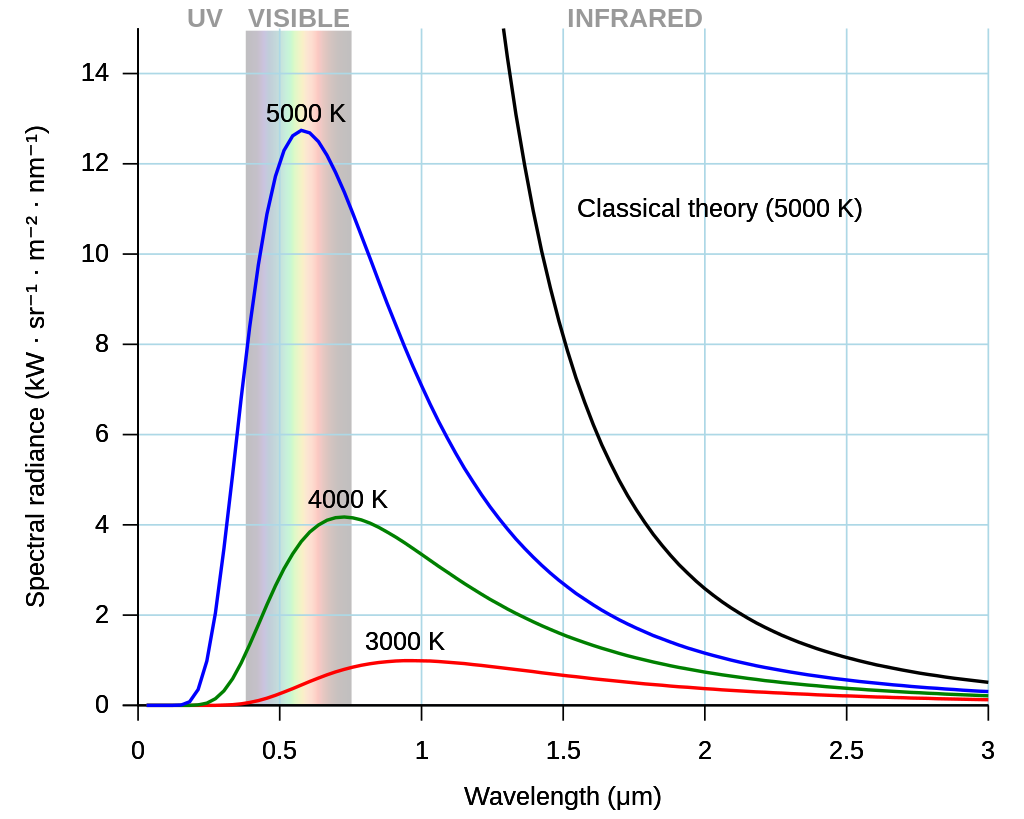
\includegraphics[width=0.35\linewidth]{../figs/methods/planck.png}
  \end{figure}
\end{frame}

\begin{frame}{Prectical Thermal Camera}
  \begin{itemize}
    \item Image intensity depends on the both the object's temperature and the camera's intrinsic (ambient) temperature:
    \begin{equation}
      \begin{split}            
          I = I(T_\mathit{obj}, T_\mathit{int})
      \end{split}
    \end{equation}
    \item Nugent et al. \cite{10.1117/1.OE.52.6.061304} suggested 3rd order polynomials for the dependency in $T_\mathit{int}$:
    \begin{equation} \label{eq:IntensityVsTemperatures}
      \begin{split}            
        I(T_\mathit{obj}, T_\mathit{int}) &= p^{(0)}_c(T_\mathit{int}) T^4_\mathit{obj} + p^{(1)}_c(T_\mathit{int})\\
        p^{(i)}_c(T_\mathit{int}) &= \sum_{k=0}^3  c_{i,k} T_\mathit{int}^k
    \end{split}
    \end{equation}
  \end{itemize}
\end{frame}

\begin{frame}{Physical UI2I (Our Contribution)}
  \begin{itemize} 
    \item Use Nugent et al.'s theorem to calibrate 2 thermal models:
    \begin{enumerate}
      \item Transform panchromatic intensities to object temperatures:
      \begin{equation*}
        \hat{T}_\mathit{obj} = \sqrt[\leftroot{5} 4]{\frac{\pmb{I_\mathit{pan}} - p^{(0)}_{c_\mathit{pan}}(\pmb{T_\mathit{pan}})}{p^{(1)}_{c_\mathit{pan}}(\pmb{T_\mathit{pan}})}}
      \end{equation*}
      \item Transform object temperatures to monochromatic intensities.
      \begin{equation*}
        \hat{I}_\mathit{mono} = p^{(1)}_{c_\mathit{mono}}(\pmb{T_\mathit{mono}}) \pmb{\hat{T}_\mathit{obj}}^4 + p^{(0)}_{c_\mathit{mono}}(\pmb{T_\mathit{mono}})
      \end{equation*}
    \end{enumerate}
    \item Cascade the transformations to get a complete panchromatic to monochromatic UI2I model.
  \end{itemize}
\end{frame}

\begin{frame}{Calibration}
  A calibration setup was designed to calibrate the coefficients from equation \ref{eq:IntensityVsTemperatures} per-pixel independently.
  \begin{figure}
    \begin{subfigure}[b]{0.49\textwidth}
        \centering
        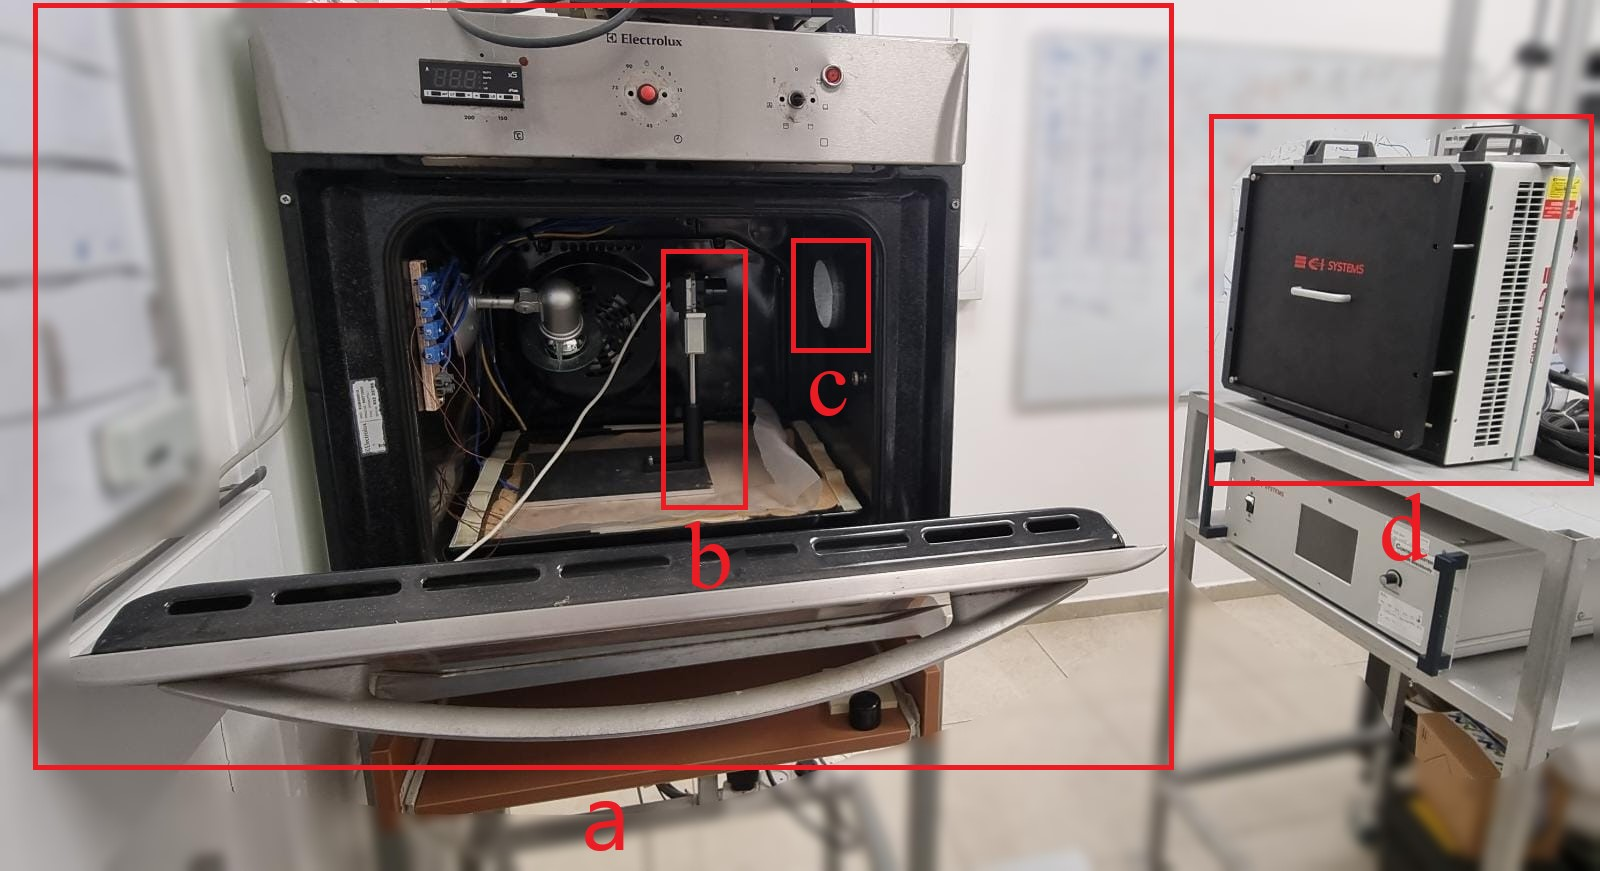
\includegraphics[width=0.9\textwidth]{../figs/methods/calib_setup.jpg}
        \subcaption*{Calibration setup}
        \label{fig:calib_setup}
    \end{subfigure}
    \hfill
    \begin{subfigure}[b]{0.49\textwidth}
        \centering
        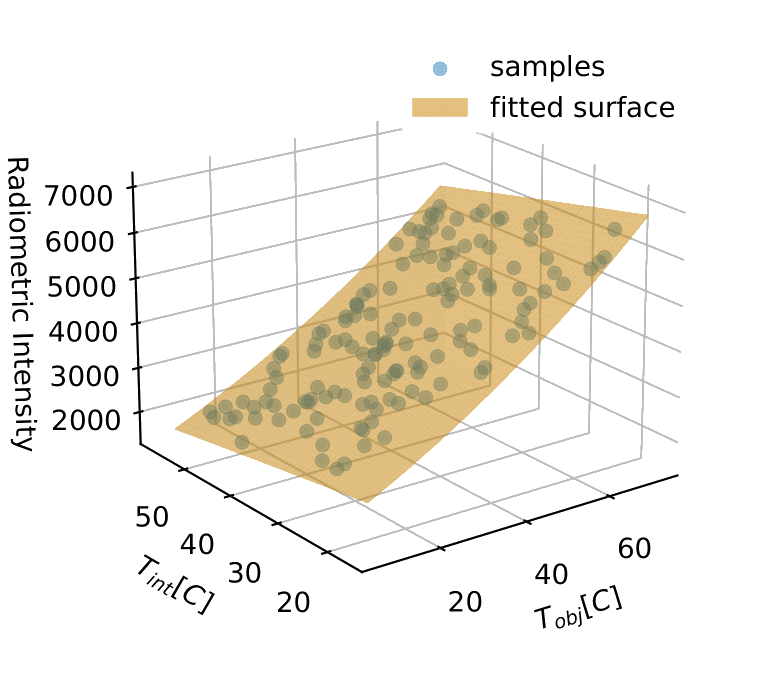
\includegraphics[width=0.9\textwidth]{../figs/methods/physical_model_tight.png}
        \subcaption*{Calibrated coefficients}
        \label{fig:calib_coeffs}
    \end{subfigure}    
  \end{figure}
\end{frame}


\subsection{PETIT}
\begin{frame}{Description}
  \begin{itemize}
    \item PETIT is a fusion of the deep generator with the physical estimators.
    \item Trained with the loss criteria and discriminators of the deep backbones as is.
  \end{itemize}
\end{frame}

\begin{frame}{Architecture}
  \begin{figure}
    \centering
    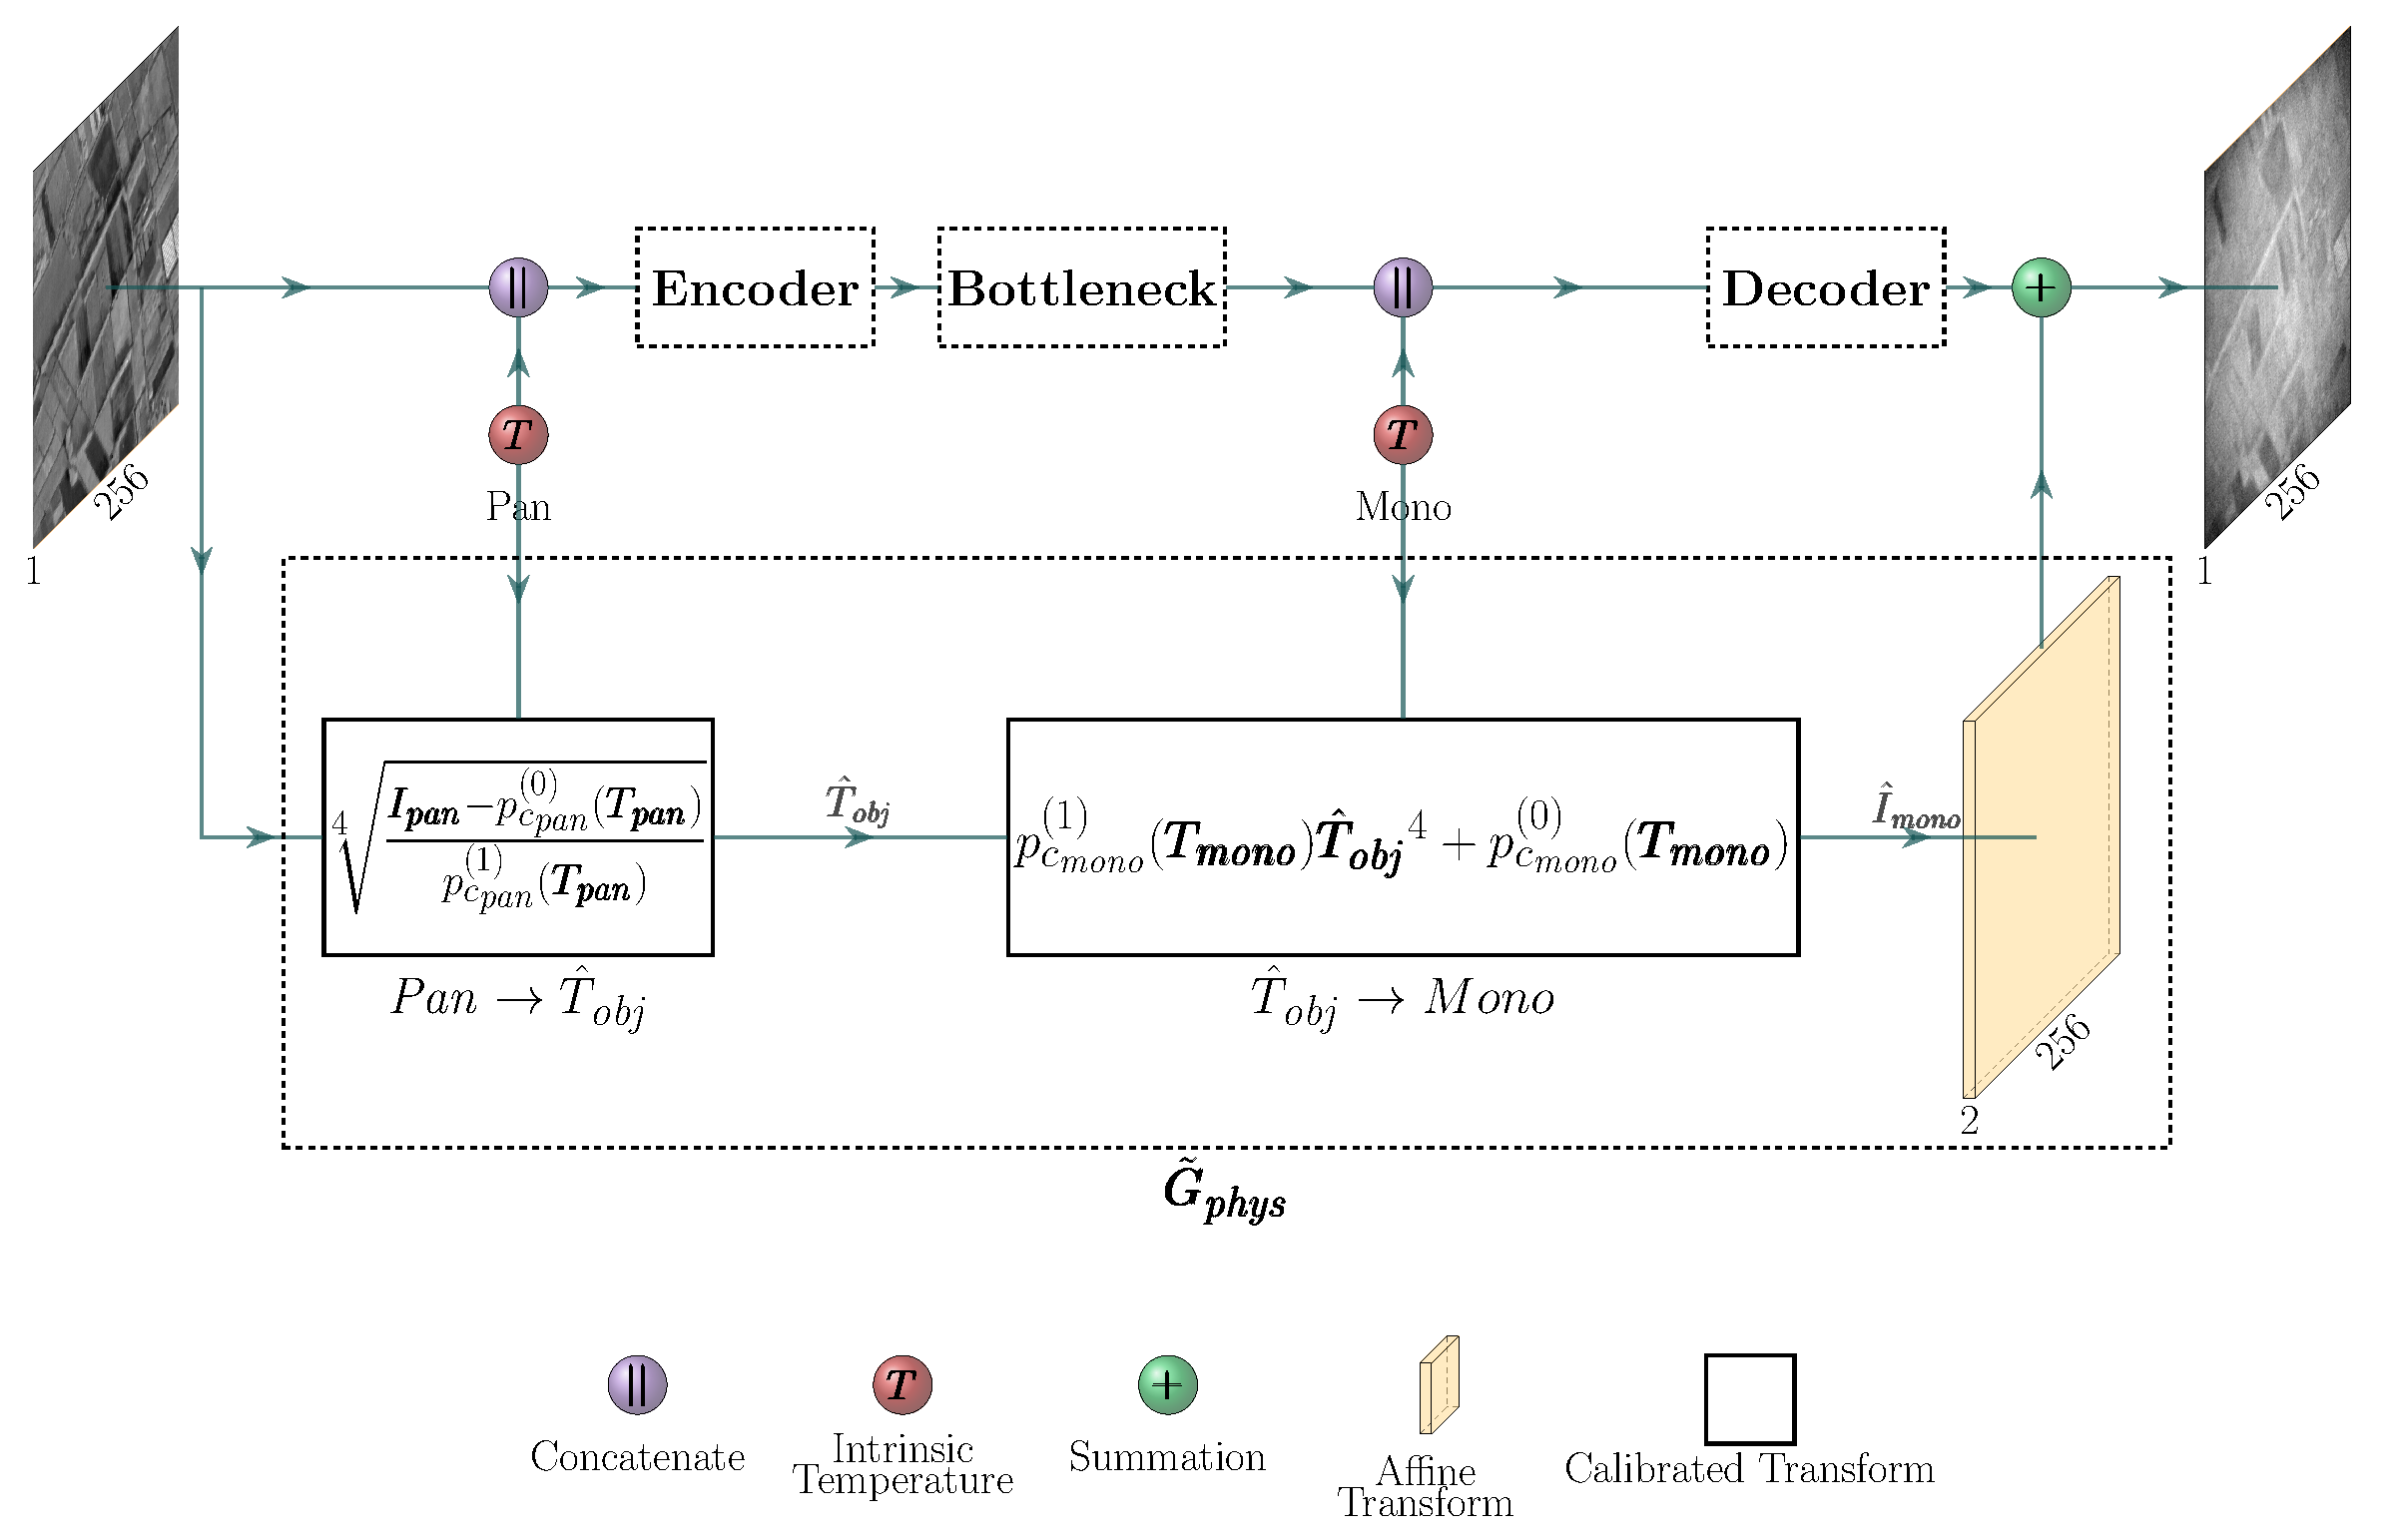
\includegraphics[width=\linewidth]{../figs/network/src/petit.pdf}
  \end{figure}
\end{frame}